\documentclass[aspectratio=169]{beamer}
\usefonttheme{serif}
\usepackage[T1]{fontenc}
\usepackage{fourier}
\usepackage{amsmath,amssymb,booktabs,graphicx,array,mathrsfs}
\usepackage{pgfpages}
\usepackage{HKUSTstyle}
\definecolor{hkustblue}{RGB}{0,56,116}
\definecolor{hkustyellow}{RGB}{167,131,55}
\definecolor{hkustred}{RGB}{209,51,59}
\setbeamertemplate{navigation symbols}{}
% Suppress automatic section-divider frames to keep exactly 19 slides.
\AtBeginSection[]{}
\AtBeginSubsection[]{}
\setbeamersize{text margin left=7mm,text margin right=7mm}
\setbeamerfont{block title}{size=\normalsize}
\setbeamerfont{block body}{size=\normalsize}
\setbeameroption{hide notes}
% Compile with \def\presenternotes{1} before \input to export notes only.
\ifdefined\presenternotes\setbeameroption{show only notes}\fi
\graphicspath{{figures/}}
\newcommand{\source}[1]{\par\vspace{1mm}{\scriptsize\color{gray}#1}}
\newcommand{\takeaway}[1]{\par\vspace{2mm}{\color{hkustblue}\textbf{#1}}}
\newcommand{\plotnote}{\source{Saved pilot: 5 replications per condition. Bars: 95\% pointwise Monte Carlo $t$ intervals.}}
\newcommand{\talknote}[2]{\note{\textbf{Target time: #1 seconds.}\par\medskip #2}}
\author{Ruijie Liu}
\title[STAT 293: Multi-VAR]{Penalized Estimation and Forecasting of Multiple Subject Intensive Longitudinal Data}
\subtitle{Multi-VAR estimation and a preliminary simulation study}
\institute{STAT 293\\University of California, Riverside}
\date{November 12, 2026}
% Keep the template footer, with a fixed presentation date on recompilation.
\renewcommand{\today}{November 12, 2026}

\begin{document}

% 1 | 0:00--0:45
\begin{frame}
\titlepage
\talknote{45}{This project studies multi-VAR, the method of Fisher and colleagues for estimating several related multivariate time series. The question is how to share information across people while retaining their individual dynamics. I will motivate the model, explain estimation, and discuss our new simulation pilot and next steps. The numerical results are our simulations, rather than a reproduction of the paper's figures.}
\end{frame}

\section{Introduction}
% 2 | 0:45--1:50
\begin{frame}{Motivation}
\begin{block}{Forecasting daily emotions}
Fisher et al. analyze daily emotion ratings from 16 people over about 11 weeks, with 20 emotion items recorded each day.
\end{block}
\vspace{2mm}
\begin{itemize}
\item A useful prediction question: how do today's emotions help predict tomorrow's emotional state?
\item Some patterns may share across people. Other patterns may differ in strength or be absent for a particular person.
\item Each person provides only about 80 daily observations, but modeling 20 emotions involves estimating 400 possible predictive relationships.
\end{itemize}
\takeaway{We want individual forecasts that can learn from other people's data.}
\end{frame}

% 3 | 1:50--2:40
\begin{frame}{Multi-VAR}
\renewcommand{\arraystretch}{1.5}
\begin{tabular}{@{}>{\raggedright\arraybackslash}p{.22\textwidth}>{\raggedright\arraybackslash}p{.32\textwidth}>{\raggedright\arraybackslash}p{.38\textwidth}@{}}
\toprule
Approach & What it estimates & Main tradeoff \\
\midrule
Individual LASSO & A separate sparse model for each person & Preserves differences, but uses little data per fit \\
Pooled LASSO & One sparse model for everyone & Shares all information, but suppresses differences \\
\textbf{Multi-VAR} & \textbf{Shared effects plus individual deviations} & \textbf{Learns how much to share through penalties} \\
\bottomrule
\end{tabular}
\takeaway{The central idea is partial sharing of dynamic relationships.}
\talknote{50}{Compare the two extremes before introducing the mathematics. Individual LASSO reduces the number of selected relationships but still fits people independently. Pooled LASSO combines the observations but assumes identical transition coefficients. Multi-VAR introduces a shared part and a separate deviation for each person. Tuning determines how expensive deviations are relative to common effects. The adaptive version will also give different coefficients different shrinkage weights.}
\end{frame}

\section{Model and methods}
% 4 | 2:40--3:50
\begin{frame}{VAR(1) model}
For subject $k=1,\ldots,K$, observe the same $d$ variables at times $t=1,\ldots,T$:
\[
\underbrace{X_t^{(k)}}_{d\times1}
=\underbrace{\Phi_1^{(k)}}_{d\times d}\,X_{t-1}^{(k)}+\varepsilon_t^{(k)},
\qquad \mathbf{B}_k^*=\operatorname{vec}\!\bigl((\Phi_1^{(k)})'\bigr)
=\boldsymbol{\mu}^*+\boldsymbol{\Delta}_k^*.
\]
\begin{itemize}
\item $\mathbf{B}_k^*$: all lag-one predictive relationships for subject $k$.
\item $\boldsymbol{\mu}^*$: a common coefficient vector shared across subjects.
\item $\boldsymbol{\Delta}_k^*$: subject $k$'s deviations from the common vector.
\end{itemize}
\end{frame}

% 5 | 3:50--4:45
\begin{frame}{Model assumptions}
\begin{itemize}
\item \textbf{Mean zero data:} the model has no intercept, center data when needed. The simulations have population mean zero.
\item \textbf{White noise:} mean zero, uncorrelated over time and with the past.
\item \textbf{Sparsity and useful sharing:} many coefficients are zero, with some recurring relationships across people.
\end{itemize}
\takeaway{Serial error correlation will test model misspecification in later simulations.}
\talknote{55}{Stability prevents the process from exploding and supports a stationary interpretation. The spectral radius is the largest absolute eigenvalue. Distinguish correlation among today's error components from correlation between today's and yesterday's errors. The former is permitted; the latter violates the innovation assumption. Gaussian innovations are the baseline simulation choice, rather than a prerequisite for writing the penalized least-squares objective. Sparsity and shared structure are the modeling motivations; recovery guarantees additionally require suitable design and signal conditions.}
\end{frame}

% 6 | 4:45--6:10
\begin{frame}{Multi-VAR estimation}
With $T_2$ training observations and $N=T_2-1$, solve
\[
\min_{\boldsymbol{\mu},\boldsymbol{\Delta}_1,\ldots,\boldsymbol{\Delta}_K}
\underbrace{\frac{1}{2KN}\sum_{k=1}^{K}
\|\mathbf{Y}^{(k)}-\mathbf{Z}^{(k)}(\boldsymbol{\mu}+\boldsymbol{\Delta}_k)\|_2^2}_{\text{prediction loss on training data}}
+\underbrace{\lambda_1\|\boldsymbol{\mu}\|_1}_{\text{shared sparsity}}
+\underbrace{\sum_{k=1}^{K}\lambda_{2,k}\|\boldsymbol{\Delta}_k\|_1}_{\text{individual sparsity}}.
\]
\vspace{2mm}
\begin{itemize}
\item Larger $\lambda_1$ discourages common effects.
\item Larger $\lambda_{2,k}$ discourages individual deviations and favors pooling.
\item Recover each subject's vector as $\widehat{\mathbf{B}}_k=\widehat{\boldsymbol{\mu}}+\widehat{\boldsymbol{\Delta}}_k$.
\end{itemize}
\talknote{85}{Read the objective in three pieces. The first asks how accurately yesterday predicts today. The common penalty encourages a small set of shared coefficients. The deviation penalty discourages unnecessary individual departures. Both are entrywise LASSO penalties. Very strong common penalization can approach independent fitting, while very strong deviation penalization can approach a pooled model. Our implementation tunes $\lambda_1$ and the ratio $r_k=\lambda_{2,k}/\lambda_1$. The loss normalization differs from the paper by a constant, which only reparameterizes the penalty scale. We evaluate the recovered total $\Phi_1^{(k)}$ matrices because they determine individual predictions.}
\end{frame}

% 7 | 6:10--7:15
\begin{frame}{Adaptive multi-VAR}
Use preliminary individual estimates $\widetilde{\mathbf{B}}_k$ and their entrywise median $\widetilde B_{\ell_j,j}$ to define weights:
\[
\omega_j=\frac{1}{|\widetilde B_{\ell_j,j}|},\qquad
\nu_{k,j}=\frac{1}{|\widetilde B_{k,j}-\widetilde B_{\ell_j,j}|}.
\]
Replace the unweighted penalties by
\[
\lambda_1\sum_j\omega_j|\mu_j|
+\sum_{k,j}\lambda_{2,k}\nu_{k,j}|\Delta_{k,j}|.
\]
\begin{itemize}
\item Large preliminary coefficients receive less shrinkage; near-zero receive more.
\item Large deviations receive less shrinkage; near-zero receive more.
\end{itemize}
\talknote{65}{Ordinary LASSO applies the same basic shrinkage to all entries. Adaptive LASSO uses a pilot to distinguish stronger and weaker candidate effects. The common pilot is the across-person median, and each deviation pilot is the difference from this median. The denominator floor keeps weights finite. In our implementation, OLS is used when the individual regression design has full rank and more rows than predictors. Otherwise a training-only standard multi-VAR pilot is used. These weights must be recomputed inside validation folds, so later observations do not influence earlier fits.}
\end{frame}

% 8 | 7:15--8:20
\begin{frame}{Computation}
Stack the subject regressions into a block design $\mathscr{Z}$ with shared and individual columns:
\[
\min_{\boldsymbol{\theta}}\;g(\boldsymbol{\theta})+\lambda_1\sum_i w_i|\theta_i|,
\qquad g(\boldsymbol{\theta})=\frac{1}{2KN}\|\mathscr{Y}-\mathscr{Z}\boldsymbol{\theta}\|_2^2.
\]
A proximal-gradient update takes a gradient step and then soft-thresholds:
\[
\begin{aligned}
\boldsymbol{\theta}^{s+1}&=\operatorname{prox}_{h,\gamma^s}
\{\boldsymbol{\theta}^s-\gamma^s\nabla g(\boldsymbol{\theta}^s)\},\\
\bigl(\operatorname{prox}_{h,\gamma^s}(\boldsymbol{\theta})\bigr)_i
&=\operatorname{sign}(\theta_i)\max\{|\theta_i|-\gamma^s\lambda_1 w_i,0\}.
\end{aligned}
\]
\talknote{65}{The shared columns use every person's observations; individual columns are active only for their subject. This turns multi-VAR into a weighted LASSO. Soft thresholding explains how exact zeros arise. FISTA accelerates a proximal-gradient method using extrapolation; the displayed equation is the basic update, not the full acceleration recursion. The adaptive method uses the same design with different weights. The custom standard solver and an independent glmnet fit agree very closely in objective value. This checks numerical optimization, not whether the scientific model assumptions hold.}
\end{frame}

% 9 | 8:20--9:20
\begin{frame}{Interpreting the estimated coefficients}
\begin{block}{An illustrative coefficient}
If $(\widehat\Phi_1^{(k)})_{ij}=0.25$, a one-unit increase in variable $j$ at the previous time predicts a $0.25$-unit increase in variable $i$ now, holding the other lagged variables fixed.
\end{block}
\begin{itemize}
\item Diagonal entries describe persistence; off-diagonal entries describe cross-variable prediction.
\item $\widehat{\boldsymbol{\mu}}$ summarizes sharing and $\widehat{\boldsymbol{\Delta}}_k$ describes departures. The penalty helps determine this decomposition.
\item A zero estimate represents a selected-out lagged predictor.
\end{itemize}
\talknote{60}{The coefficient example is hypothetical and uses the measurement units of the variables. Standardized variables would instead use standard-deviation units. An arrow in a fitted network represents a conditional lagged association. It does not establish that intervening on one emotion changes another. Also, moving a coefficient between $\boldsymbol{\mu}$ and every $\boldsymbol{\Delta}_k$ can leave the total $\mathbf{B}_k$ unchanged; the penalty selects a decomposition. Therefore this pilot evaluates total subject matrices rather than claiming unique recovery of a scientifically defined common network.}
\end{frame}

\section{Numerical experiments}
% 10 | 9:20--10:25
\begin{frame}{Baseline Simulation}
\begin{itemize}
\item $K=10$ subjects, $d=20$ variables, $T=100$ observations.
\item Per subject: 20 nonzero coefficients, with 10 common and 10 unique.
\item Positive initial coefficients from $\mathrm{Uniform}(0.1,0.9)$.
\item Gaussian iid errors with covariance $I_d$.
\item Discard 500 burn-in observations.
\end{itemize}
\talknote{65}{The baseline resembles the paper's sparse common-plus-unique construction. The common positions and each person's unique positions are disjoint, including across individual unique supports. All coefficients start positive. Multiplying every subject matrix by one scalar preserves exactly shared values and ensures stability. The final nonzero magnitudes need not remain between 0.1 and 0.9. This differs from the paper's rejection sampling. The series start at zero and use a finite burn-in to approximate stationarity. The figure shows the same variable for two simulated subjects; it is not the real emotion dataset.}
\end{frame}

% 11 | 10:25--11:15
\begin{frame}{Simulation Design}
\centering
\renewcommand{\arraystretch}{1.18}
\begin{tabular}{@{}ll@{}}
\toprule
Factor & Values tested (baseline in bold) \\
\midrule
Errors standard deviation & $0.5,\;\mathbf{1},\;2$ \\
Number of variables & $10,\;\mathbf{20},\;30,\;40$ \\
Nonzero fraction & $0.025,\;\mathbf{0.05},\;0.10,\;0.15$ \\
Same-time error correlation & $\mathbf{0},\;0.3,\;0.6$ \\
Serial error correlation & $\mathbf{0},\;0.3,\;0.6$ \\
Measurement error standard deviation & $\mathbf{0},\;0.5,\;1$ \\
Number of observations & $50,\;\mathbf{100}$ \\
\bottomrule
\end{tabular}
\vspace{3mm}
\begin{itemize}
\item Sixteen conditions, one factor at a time.
\item Five replications per condition, four estimators on each dataset.
\item Baseline reused across comparisons.
\end{itemize}
\talknote{50}{Only one factor changes from baseline at a time, giving 16 unique conditions in total. This does not estimate interactions. Contemporaneous correlation uses a Toeplitz covariance, so entries decay with variable separation. Serial innovations follow an AR(1) process while preserving their marginal variance. Measurement error is independent Gaussian noise added to the latent series. Seeds are paired across conditions where possible. Five replications are enough to inspect the workflow and suggest patterns, but too few for broad rankings.}
\end{frame}

% 12 | 11:15--12:30
\begin{frame}{Training and Test}
\begin{columns}[T]
\begin{column}{.49\textwidth}
\textbf{Training and Test}
\begin{itemize}
\item Test: Reserve the final 3 observations.
\item Within training: 5 expanding-window validation origins used for choosing penalty.
\item Refit on all training data, then forecast the final 3 observations recursively.
\end{itemize}
\end{column}
\begin{column}{.49\textwidth}
\textbf{Evaluation targets}
\[
\text{Relative error}=\frac1K\sum_k
\frac{\|\widehat\Phi_1^{(k)}-\Phi_1^{(k)}\|_F}{\|\Phi_1^{(k)}\|_F}.
\]
\begin{itemize}
\item \textbf{RMSFE:} root mean squared forecast error within person, then average across people.
\item \textbf{Sensitivity / specificity:} recovery of nonzero / zero entries.
\end{itemize}
\end{column}
\end{columns}
\talknote{75}{At baseline, observations 1 through 97 are available for training, and observations 98 through 100 remain untouched until evaluation. Each validation fit sees only a time prefix. Penalty fractions range from one to 0.001 of $\lambda_{1,\max}$, and deviation-to-common ratios are 0.05, 0.2 and 0.8 for ten subjects. Pilot weights and $\lambda_{1,\max}$ are recalculated within each prefix. Test forecasts do not feed actual test values back into the recursion. Relative Frobenius error is the main structural metric. Support uses an absolute coefficient threshold of 1e-5. Measurement-noise forecasts are scored against noisy observations, while coefficient errors target latent $\Phi_1^{(k)}$. Plot bars are pointwise Monte Carlo t intervals, not confidence intervals for a fitted person's network.}
\end{frame}

% 13 | 12:30--13:45
\begin{frame}{Baseline: sharing improves coefficient recovery}
\centering
\renewcommand{\arraystretch}{1.35}
\begin{tabular}{@{}lcc@{}}
\toprule
Method & Relative coefficient error & One-step RMSFE \\
\midrule
Individual LASSO & $0.397\;(0.016)$ & $1.056\;(0.025)$ \\
Pooled LASSO & $0.714\;(0.018)$ & $1.147\;(0.034)$ \\
Multi-VAR & $0.329\;(0.027)$ & $1.047\;(0.025)$ \\
Adaptive multi-VAR & $\mathbf{0.265}\;(0.027)$ & $1.047\;(0.027)$ \\
\bottomrule
\end{tabular}
\vspace{2mm}
\begin{itemize}
\item Multi-VAR's mean relative error is \textbf{17\% lower} than individual LASSO's; adaptive multi-VAR's is \textbf{33\% lower}.
\item Forecast differences among the three individualized methods are small.
\end{itemize}
\talknote{75}{The main baseline result is stronger recovery of coefficients when the data contain shared structure. Pooled LASSO loses the individual component and has the largest coefficient error. The percentages compare the mean relative errors, not each person's percentage improvement. Paired differences compare methods on the same simulated dataset and account for that dependence. Forecasting tells a weaker story: standard and adaptive multi-VAR have almost identical average one-step RMSFE, and both are close to individual LASSO. The paired forecast differences from individual LASSO are about minus 0.0084, with SEs 0.0055 and 0.0089. Avoid claiming a clear forecast winner from this pilot.}
\end{frame}

% 14 | 13:45--14:50
\begin{frame}{Dimension and density affect recovery}
\centering
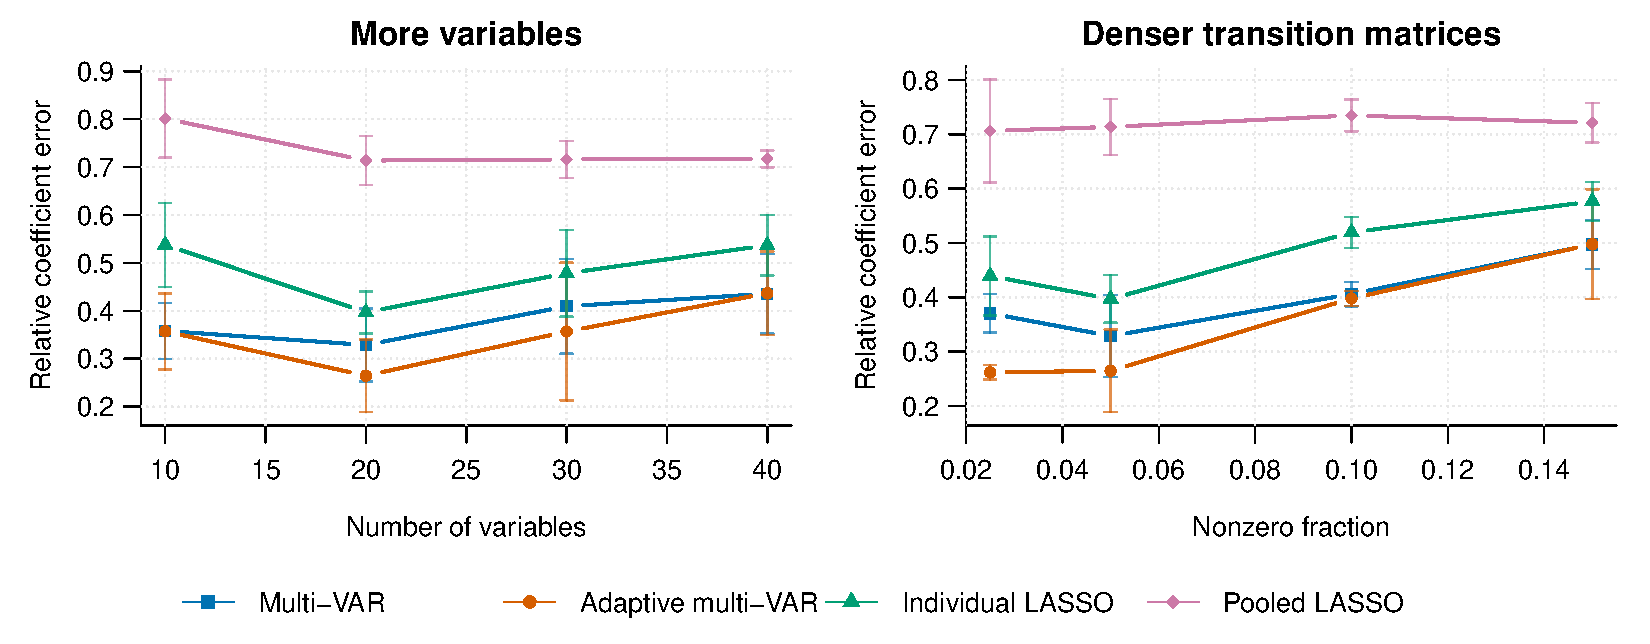
\includegraphics[width=\textwidth]{dimension_density.pdf}
\talknote{65}{Read lower values as better. From 20 to 40 variables the problem becomes harder, but dimension ten does not simply continue a monotonic trend. At fixed density, changing d also changes the number of active coefficients; at d ten, rounding makes the common fraction 0.4 rather than exactly 0.5. Denser matrices also require a different rescaling to enforce the same maximum spectral radius. Thus these are results for this construction, not pure effects of dimension or sparsity at fixed effect magnitude. The shorter-series condition, not plotted here, has higher coefficient error. Its forecast error does not have to increase monotonically in a small pilot with different forecast targets.}
\end{frame}

% 15 | 14:50--16:15
\begin{frame}{Serial correlation disrupts recovery}
\centering
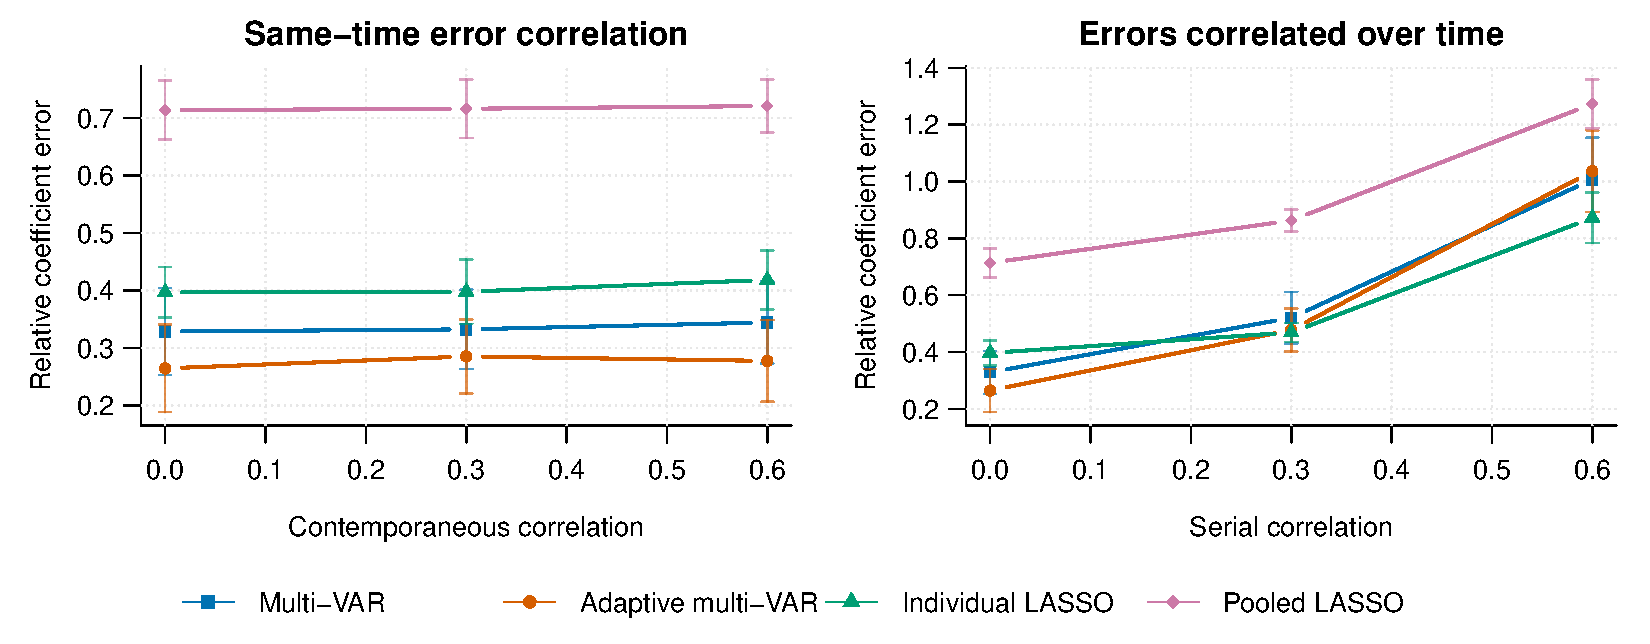
\includegraphics[width=\textwidth]{dependence.pdf}
\talknote{85}{The two panels separate two distinct forms of error dependence. Serially correlated errors are related to lagged outcomes, so the fitted VAR(1) coefficients can absorb predictable error dynamics instead of recovering the structural $\Phi_1^{(k)}$. The improvement in one-step RMSFE is therefore not evidence of improved structural estimation. The marginal error variance is held fixed as serial correlation changes, but the conditional predictability changes. At serial correlation 0.6, individual LASSO's mean coefficient error is 0.872 compared with multi-VAR's 1.007 and adaptive multi-VAR's 1.036. The baseline ordering is therefore not universal. This is an explicit robustness experiment under misspecification.}
\end{frame}

% 16 | 16:15--17:20
\begin{frame}{Measurement error disrupts recovery}
\centering
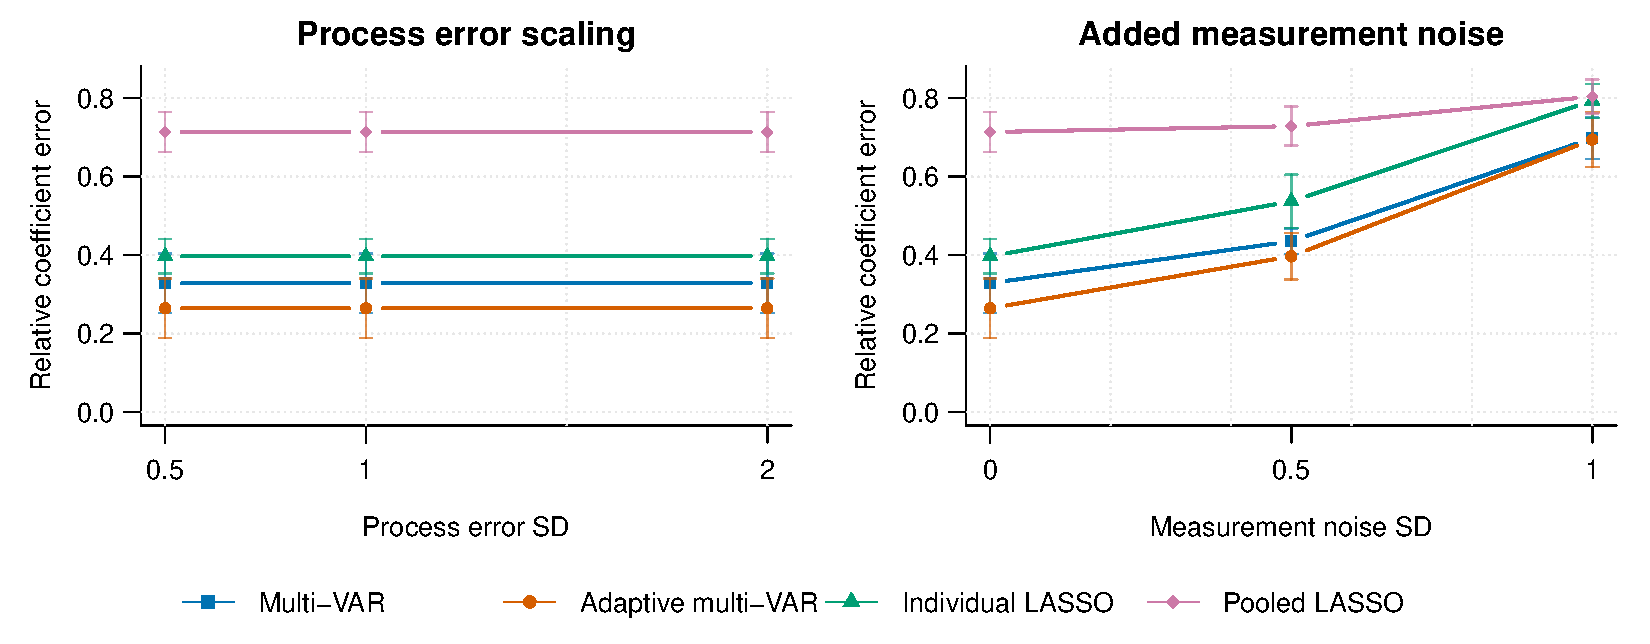
\includegraphics[width=\textwidth]{scale_measurement.pdf}

\talknote{65}{Both panels now measure relative coefficient error on the same vertical scale. This distinction prevents a misleading interpretation of noise experiments. If innovations are multiplied by sigma, the entire latent process scales with sigma. Both predictors and responses scale, and our penalty grid adjusts accordingly. The saved paired runs have identical coefficient errors across innovation scales, while forecast errors scale exactly. Normalizing RMSFE by sigma removes that scale change. In contrast, independent measurement error contaminates the observed predictor and response without similarly scaling the underlying signal. This creates an errors-in-variables problem and worsens recovery of the latent transition matrix.}
\end{frame}

% 17 | 17:20--18:25
\begin{frame}{Adaptive shrinkage trades sensitivity for specificity}
\centering
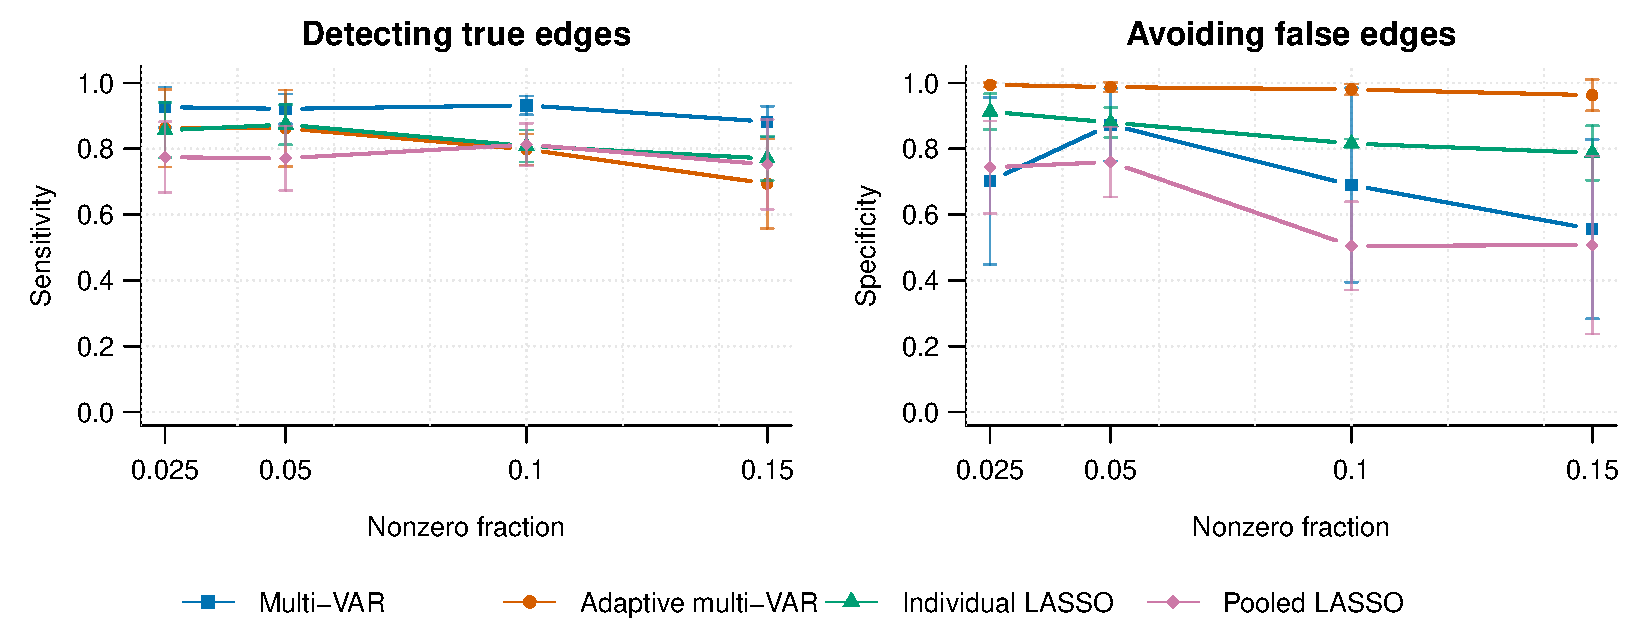
\includegraphics[width=\textwidth]{support.pdf}

\talknote{65}{Both panels vary the nonzero fraction and use the same vertical scale. Higher nonzero fractions mean denser true networks. The left panel shows sensitivity, the proportion of true edges recovered. The right panel shows specificity, the proportion of true zero entries correctly left at zero. At 15 percent density, standard multi-VAR has sensitivity 0.882 versus 0.694 for adaptive multi-VAR, but specificity 0.556 versus 0.963. This illustrates the tradeoff: adaptive fitting avoids more false edges but misses more true edges. These are pilot results under our stability-rescaled construction; increasing density also changes coefficient magnitudes, so this is not a pure density effect at fixed signal strength. Support is evaluated on total subject matrices. Values and intervals summarize replication-level averages across subjects. The pointwise t intervals may extend beyond the zero-to-one range.}
\end{frame}

\section{Future steps}
% 18 | 18:25--19:30
\begin{frame}{Future steps}
\begin{enumerate}
\item \textbf{Strengthen the numerical comparison}\newline
Increase to 20--50 replications; Use more validation origins.
\vspace{2mm}
\item \textbf{Connect prediction to a real application}\newline
Check method performence in a real dataset.

First choice for now: FLIP is a daily diary study of personality, emotions, and motivation. Participants reported how they felt and behaved each day over an 82-day period.

\end{enumerate}
\talknote{65}{These are proposed next analyses, not completed results. First, improve Monte Carlo precision and tuning coverage. The ratio boundary rates suggest checking a wider or finer grid, although choosing a boundary can legitimately favor pooled or independent fitting. Second, vary the degree of sharing directly and separate dimension from active coefficient count. Signed coefficients and more realistic heterogeneity would test beyond the current positive, disjoint support construction. Finally, apply the approach to actual emotion data if accessible, with careful preprocessing and a time-ordered test set. Serial dependence suggests investigating additional lags or explicit error dynamics rather than interpreting the current fitted matrix causally.}
\end{frame}

% 19 | 19:30--20:00
\begin{frame}{Reference}

\vspace{3mm}
{\small\textbf{Reference}\\
Fisher, Z. F., Kim, Y., Fredrickson, B. L., \& Pipiras, V. (2022).\\
\emph{Penalized Estimation and Forecasting of Multiple Subject Intensive Longitudinal Data}. Psychometrika, 87, 403--431.\\
\href{https://doi.org/10.1007/s11336-021-09825-7}{doi:10.1007/s11336-021-09825-7}}
\par\vspace{3mm}
\talknote{30}{Close by returning to the original motivation: use other people's information without erasing individual differences. In the pilot, this helps recover coefficients when the assumed structure is appropriate. Forecasting and structural interpretation are different targets, particularly under serially correlated innovations. The next stage is a larger, better-tuned robustness study and a carefully checked real-data application. Invite questions.}
\end{frame}

\end{document}
